\section{$\mathbf{X}=\mathbf{W}\mathbf{H}$ Non-Negative Matrix Factorization}

Non-Negative Matrix Factorization (NNMF) is a linear dimensionality reduction and blind source detection technique for positive data. It has a reputation of generating decompositions that are "sparse and meaningful". 

Following the convention in \citeasnoun{gillis2014nonnegative}, it works by expressing a positive data matrix $\mathbf{X}\in\mathbb{R}^{p\times n}_+$ in terms of two smaller positive matrices $\mathbf{W}\in\mathbb{R}_+^{p\times r}$ and $\mathbf{H}\in \mathbb{R}^{r\times n}_+$. Here the $n$ columns of the data matrix are data points and the rows are the $p$ features. An excellent introduction to NNMF is found in \possessivecite{morningpaper2019nnmf} blog post and in \citeasnoun{gillis2014nonnegative}. Dimensionality reduction derives from the ability to adjust the rank of the decomposition via the dimension $r$. The decomposition is simply:

\begin{equation}
\mathbf{X} \approx \mathbf{WH}
\end{equation}

Where the error $||\mathbf{X} - \mathbf{WH}||_\alpha$ is minimized with respect to some norm (normally, the Frobenius norm with $\alpha=2$). The decomposition allows the interpretation of $\mathbf{W} \in \mathbb{R}^{p\times r}$ as a matrix with a number of $r$ $p$-dimensional strictly positive basis vectors and of $\mathbf{H} \in \mathbb{R}^{r\times n}$ as a matrix of coefficients that express the $n$ data points in terms of linear sums of the $r$ basis vectors with strictly positive coefficients. 

One might ask: why NNMF when I can create linear decompositions of my data with SVD and PCA? After all, these techniques are well established and are known to give the optimal approximation under the Frobenius nurm. In my perception, the key difference is that NNMF solves the constrained problem of forcing both coefficients and basis vectors to be strictly positive. For many data types, negative values (word frequencies, pixel values) are unnatural, and so the results of NNMF are immediately more interpretable. NNMF is promising in particular in situations where a signal arises from the addition of a number of positive signals. A canonical example is hyperspectral imaging, where, assuming incoherent light, the measured spectrum is the linear sum of the spectra of the individual light sources. If all goes well, the basis vectors from NNMF of a hyperspectral image will be the source spectra. In the context of natural language processing, NNMF on a collection of documents can be interpreted as \textit{topics}. Figure \ref{fig:nnmf_eigenfaces} shows the NNMF-based decomposition and approximation of the "labeled faces in the wild" dataset, analogous to the SVD of the dataset shown in Figure \ref{fig:svd_eigenfaces}. The two are quite different. While for SVD, the faces look as if they are gradually coming into focus, for NNMF the faces are at first not recognizable. The portraits also become brighter in the plot as more basis components are added, because, in contrast to the SVD case, the composition is purely additive.  

The drawback is that NNMF is computationally more difficult (possibly NP hard), nor is the matrix approximation optimal, nor is the decomposition unique. 


\begin{figure}
\centering
    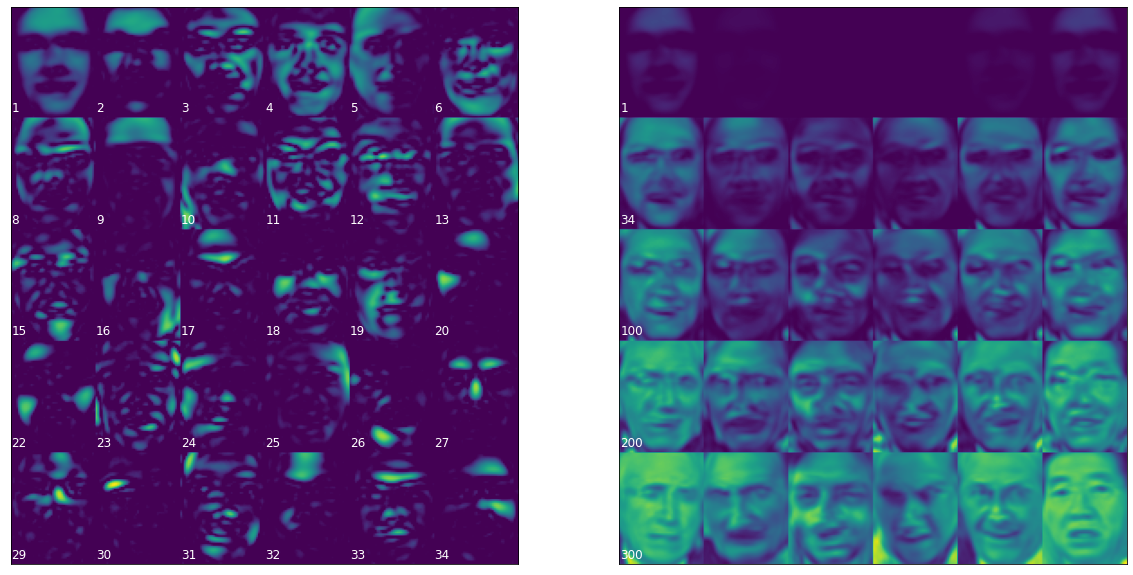
\includegraphics[width=\textwidth]{nnmf_eigenfaces.png}
    \caption{Left: The first 48 basis faces extracted using NNMF under frobenius norm from the "Labeled Faces in the Wild" Dataset. The basis images are normalized and shown on a log scale because they have very different contrast and brightness. The normalized images are then all shown on the same color scale. Right: Five sample portraits from the dataset approximated using different numbers of basis faces. The NNMF was done for a value of $r=300$. The original portraits had $2914$ pixels.}
    \label{fig:svd_eigenfaces}
\end{figure}